\documentclass[aspectratio=169]{beamer}

\usepackage[utf8]{inputenc}
\usepackage[T1]{fontenc}
\usepackage[brazil]{babel}
\usepackage{ragged2e}
\usepackage{booktabs}
\usepackage{verbatim}

%%\usetheme{AnnArbor}
\usecolortheme{orchid}
\usefonttheme[onlymath]{serif}

\AtBeginSection[]{
  \begin{frame}
  \vfill
  \centering
  \begin{beamercolorbox}[sep=8pt,center,shadow=true,rounded=true]{title}
    \usebeamerfont{title}\insertsectionhead\par%
  \end{beamercolorbox}
  \vfill
  \end{frame}
}

\title[\sc{Programação Orientada a Objetos - ECo}]{Programação Orientada a Objetos - ECo}
\author[Mangan \and Teodorowitsch]{Marco Mangan \and Roland Teodorowitsch}

\institute[POO-ECo - ECo - PUCRS]{Programação Orientada a Objetos \\ Engenharia de Computação \\
Pontifícia Universidade Católica do Rio Grande do Sul}
\date{5 de agosto de 2024}

\begin{document}
\justifying


\begin{frame}
	\titlepage
\end{frame}


\section{Apresenta\c{c}\~ao do Professor}


\begin{frame}\frametitle{Sobre o professor}
    \begin{itemize}
    	\item Nome:
    		\begin{itemize}
    			\item Marco Mangan
    		\end{itemize}
    	\item Forma\c{c}\~ao:
    		\begin{itemize}
    			\item Bel. em Ci\^encia da Computa\c{c}\~ao (UFRGS, 1996)
    			\item MSc. em Ci\^encia da Computa\c{c}\~ao (UFRGS, 1998)
       			\item DSc. em Engenharia de Sistemas e Computa\c{c}\~ao (UFRJ, 2006)
    		\end{itemize}
    	\item \'Areas de Interesse:
    		\begin{itemize}
    			\item Linguagens de Programação
                \item Engenharia de Software
    		\end{itemize}
    	%\item Correio eletrônico:
    	%	\begin{itemize}
    	%		\item marco.mangan@pucrs.br
    	%	\end{itemize}
    \end{itemize}
\end{frame}

\section{Apresenta\c{c}\~ao dos 
Estudantes}

\begin{frame}\frametitle{Sobre você}
    \begin{itemize}
    	\item O que espera da disciplina?
    	\item Já realiza estágio ou trabalha com programação?
    	\item Gostaria de trabalhar com programação?
     	\item Já programa em orientação a objetos?
    	\item Já programa em C++?
    	\item Qual seria o maior impedimento nesta disciplina?    
    \end{itemize}
\end{frame}

\section{Motivos para estudar C++}

\begin{frame}
    \frametitle{Aplicações do Mundo Real em C++ (1/2)}

    \begin{itemize}
        \item \textbf{LibreOffice}
        \begin{itemize}
            \item Suíte de escritório com processamento de texto, planilhas e mais.
            \item Uso extensivo de princípios de programação orientada a objetos.
            \item \href{https://github.com/LibreOffice/core}{https://github.com/LibreOffice/core}
        \end{itemize}

        \item \textbf{VLC Media Player}
        \begin{itemize}
            \item Reprodutor de mídia multiplataforma suportando vários formatos.
            \item Demonstra padrões de design e processamento multimídia.
            \item \href{https://code.videolan.org/videolan/vlc}{https://code.videolan.org/videolan/vlc}
        \end{itemize}
    \end{itemize}
\end{frame}

\begin{frame}

\frametitle{Aplicações do Mundo Real em C++ (2/2)}

    \begin{itemize}
        \item \textbf{Qt}
        \begin{itemize}
            \item Ferramenta para criação de interfaces gráficas de usuário.
            \item Enfatiza hierarquias de classes e programação orientada a eventos.
            \item \href{https://github.com/qt/qtbase}{https://github.com/qt/qtbase}
        \end{itemize}

        \item \textbf{LLVM}
        \begin{itemize}
            \item Tecnologias de compiladores e ferramentas modulares e reutilizáveis.
            \item Demonstra arquitetura modular e design orientado a objetos.
            \item \href{https://github.com/llvm/llvm-project}{https://github.com/llvm/llvm-project}
        \end{itemize}

        \item \textbf{V8}
        \begin{itemize}
            \item Motor de JavaScript e WebAssembly de alto desempenho.
            \item Usa C++ para aplicações onde o desempenho é crítico.
            \item \href{https://github.com/v8/v8}{https://github.com/v8/v8}
        \end{itemize}
    \end{itemize}
\end{frame}

\begin{frame}
    \frametitle{Principais Empresas no Mundo que Contratam Desenvolvedores C++}

    \small
    \begin{tabular}{p{0.3\textwidth} p{0.6\textwidth}}
        \textbf{Google} & 
        Indústria: Tecnologia \\
        & Uso de C++: Motor de busca, navegador Chrome, ferramentas internas \\
        & \href{https://www.google.com}{https://www.google.com}  \\ \hline
        
        \textbf{Microsoft} & 
        Indústria: Tecnologia \\
        & Uso de C++: Windows OS, Microsoft Office, Visual Studio \\
        & \href{https://www.microsoft.com}{https://www.microsoft.com} \\ \hline
        
        \textbf{Amazon} & 
        Indústria: E-commerce e Computação em Nuvem \\
        & Uso de C++: Infraestrutura AWS, software de dispositivos Kindle \\
        & \href{https://www.amazon.com}{https://www.amazon.com} \\ \hline
        
        \textbf{Apple} & 
        Indústria: Tecnologia \\
        & Uso de C++: MacOS, iOS, Safari, Final Cut Pro \\
        & \href{https://www.apple.com}{https://www.apple.com} \\
    \end{tabular}
\end{frame}

\begin{frame}
    \frametitle{Mais Empresas Internacionais Contratando Desenvolvedores C++}

    \small
    \begin{tabular}{p{0.3\textwidth} p{0.6\textwidth}}
        \textbf{Intel} & 
        Indústria: Semicondutores \\
        & Uso de C++: Drivers, firmware, computação de alto desempenho \\
        & \url{https://www.intel.com} \\ \hline
        
        \textbf{NVIDIA} & 
        Indústria: Gráficos e IA \\
        & Uso de C++: GPUs, CUDA para computação paralela \\
        & \url{https://www.nvidia.com} \\ \hline
        
        \textbf{Bloomberg} & 
        Indústria: Serviços Financeiros \\
        & Uso de C++: Processamento de dados financeiros, análises em tempo real \\
        & \url{https://www.bloomberg.com} \\ \hline
        
        \textbf{Goldman Sachs} & 
        Indústria: Serviços Financeiros \\
        & Uso de C++: Plataformas de negociação, gestão de riscos \\
        & \url{https://www.goldmansachs.com} \\
    \end{tabular}
\end{frame}

\begin{frame}
    \frametitle{Empresas Adicionais que Contratam Desenvolvedores C++}

    \small
    \begin{tabular}{p{0.3\textwidth} p{0.6\textwidth}}
        \textbf{Electronic Arts (EA)} & 
        Indústria: Jogos \\
        & Uso de C++: Desenvolvimento de jogos, aplicações multiplataforma \\
        & \url{https://www.ea.com} \\ \hline
        
        \textbf{Siemens} & 
        Indústria: Industrial e Engenharia \\
        & Uso de C++: Automação, sistemas de controle, soluções embarcadas \\
        & \url{https://www.siemens.com} \\
    \end{tabular}
\end{frame}

\begin{frame}
    \frametitle{Principais Empresas no Brasil que Contratam Desenvolvedores C++}

    \small
    \begin{tabular}{p{0.3\textwidth} p{0.6\textwidth}}
        \textbf{Embraer} & 
        Indústria: Aeroespacial \\
        & Uso de C++: Sistemas aviônicos, software de controle de voo \\
        &  \url{https://www.embraer.com} \\ \hline
        
        \textbf{TOTVS} & 
        Indústria: Software \\
        & Uso de C++: Desenvolvimento de software ERP \\
        & \url{https://www.totvs.com} \\ \hline
        
        
        \textbf{Stefanini} & 
        Indústria: Serviços de TI \\
        & Uso de C++: Desenvolvimento de software, consultoria \\
        &  \url{https://www.stefanini.com} \\
    \end{tabular}
\end{frame}

\begin{frame}
    \frametitle{Mais Empresas Brasileiras Contratando Desenvolvedores C++}

    \small
    \begin{tabular}{p{0.3\textwidth} p{0.6\textwidth}}
        \textbf{Dell Technologies} & 
        Indústria: Tecnologia \\
        & Uso de C++: Soluções de hardware, serviços em nuvem \\
        & \url{https://www.dell.com} \\ \hline
        
        \textbf{Movile} & 
        Indústria: Serviços Móveis \\
        & Uso de C++: Aplicativos móveis e plataformas \\
        &  \url{https://www.movile.com} \\ \hline
        
        \textbf{CINQ Technologies} & 
        Indústria: Serviços de TI \\
        & Uso de C++: Software personalizado para automotivo e manufatura \\
        & \url{https://www.cinq.com.br} \\ \hline
        
        \textbf{Samsung Research Brazil} & 
        Indústria: Tecnologia \\
        & Uso de C++: Tecnologias móveis, eletrônicos de consumo \\
        & \url{https://research.samsung.com} \\
    \end{tabular}
\end{frame}

\begin{frame}
    \frametitle{Empresas Adicionais no Brasil Contratando Desenvolvedores C++}

    \small
    \begin{tabular}{p{0.3\textwidth} p{0.6\textwidth}}
        \textbf{Itaú} & 
        Indústria: Serviços Financeiros \\
        & Uso de C++: Sistemas bancários, gestão de riscos \\
        & \url{https://www.itau.com.br} \\ \hline
        
        \textbf{Petrobras} & 
        Indústria: Energia \\
        & Uso de C++: Simulação, modelagem para exploração e produção \\
        & \url{https://petrobras.com.br} \\
    \end{tabular}
\end{frame}

\section{Apresenta\c{c}\~ao da Disciplina}


\begin{frame}\frametitle{Sobre a disciplina}
\begin{itemize}
	\item Nome: Programação Orientada a Objetos - ECo
	\item Código: 98718-04
	\item Turma: 10
	\item Cr\'editos: 4
	\item Carga-horária: 60 horas-aula
	\item Hor\'ario:
	\begin{itemize}
		%\item Turma 10: 2AB 4AB (AB=8h-9h30min)
		\item Turma 11: 2CD 4CD (Segundas e quartas-feiras, das 9h45 às 11h15)
	\end{itemize}
	\item Modalidade: presencial
\end{itemize}
\end{frame}


\begin{frame}\frametitle{Sobre a disciplina}
\begin{itemize}
	\item Semestre: 2
	\item Pré-requisito:
		\begin{itemize}
			\item Introdução à Programação - ECo
		\end{itemize}
	\item Co-requisito:
		\begin{itemize}
			\item Algoritmos e Estruturas de Dados I
		\end{itemize}
	\item Pré-requisito para:
		\begin{itemize}
			\item Fundamentos de Processamento Paralelo e Distribuído
		\end{itemize}
\end{itemize}
\end{frame}

%{%
%\usebackgroundtemplate{
%  \centering
%  \includegraphics[width=\paperwidth]{pucrs-ec-poo-unidade_00-apresentacao_da_disciplina-laminas-matriz_curricular.jpg}
%}
%\begin{frame}\frametitle{}
%\end{frame}
%}

\begin{frame}[plain] % The 'plain' option removes default header/footer
    \begin{center}
        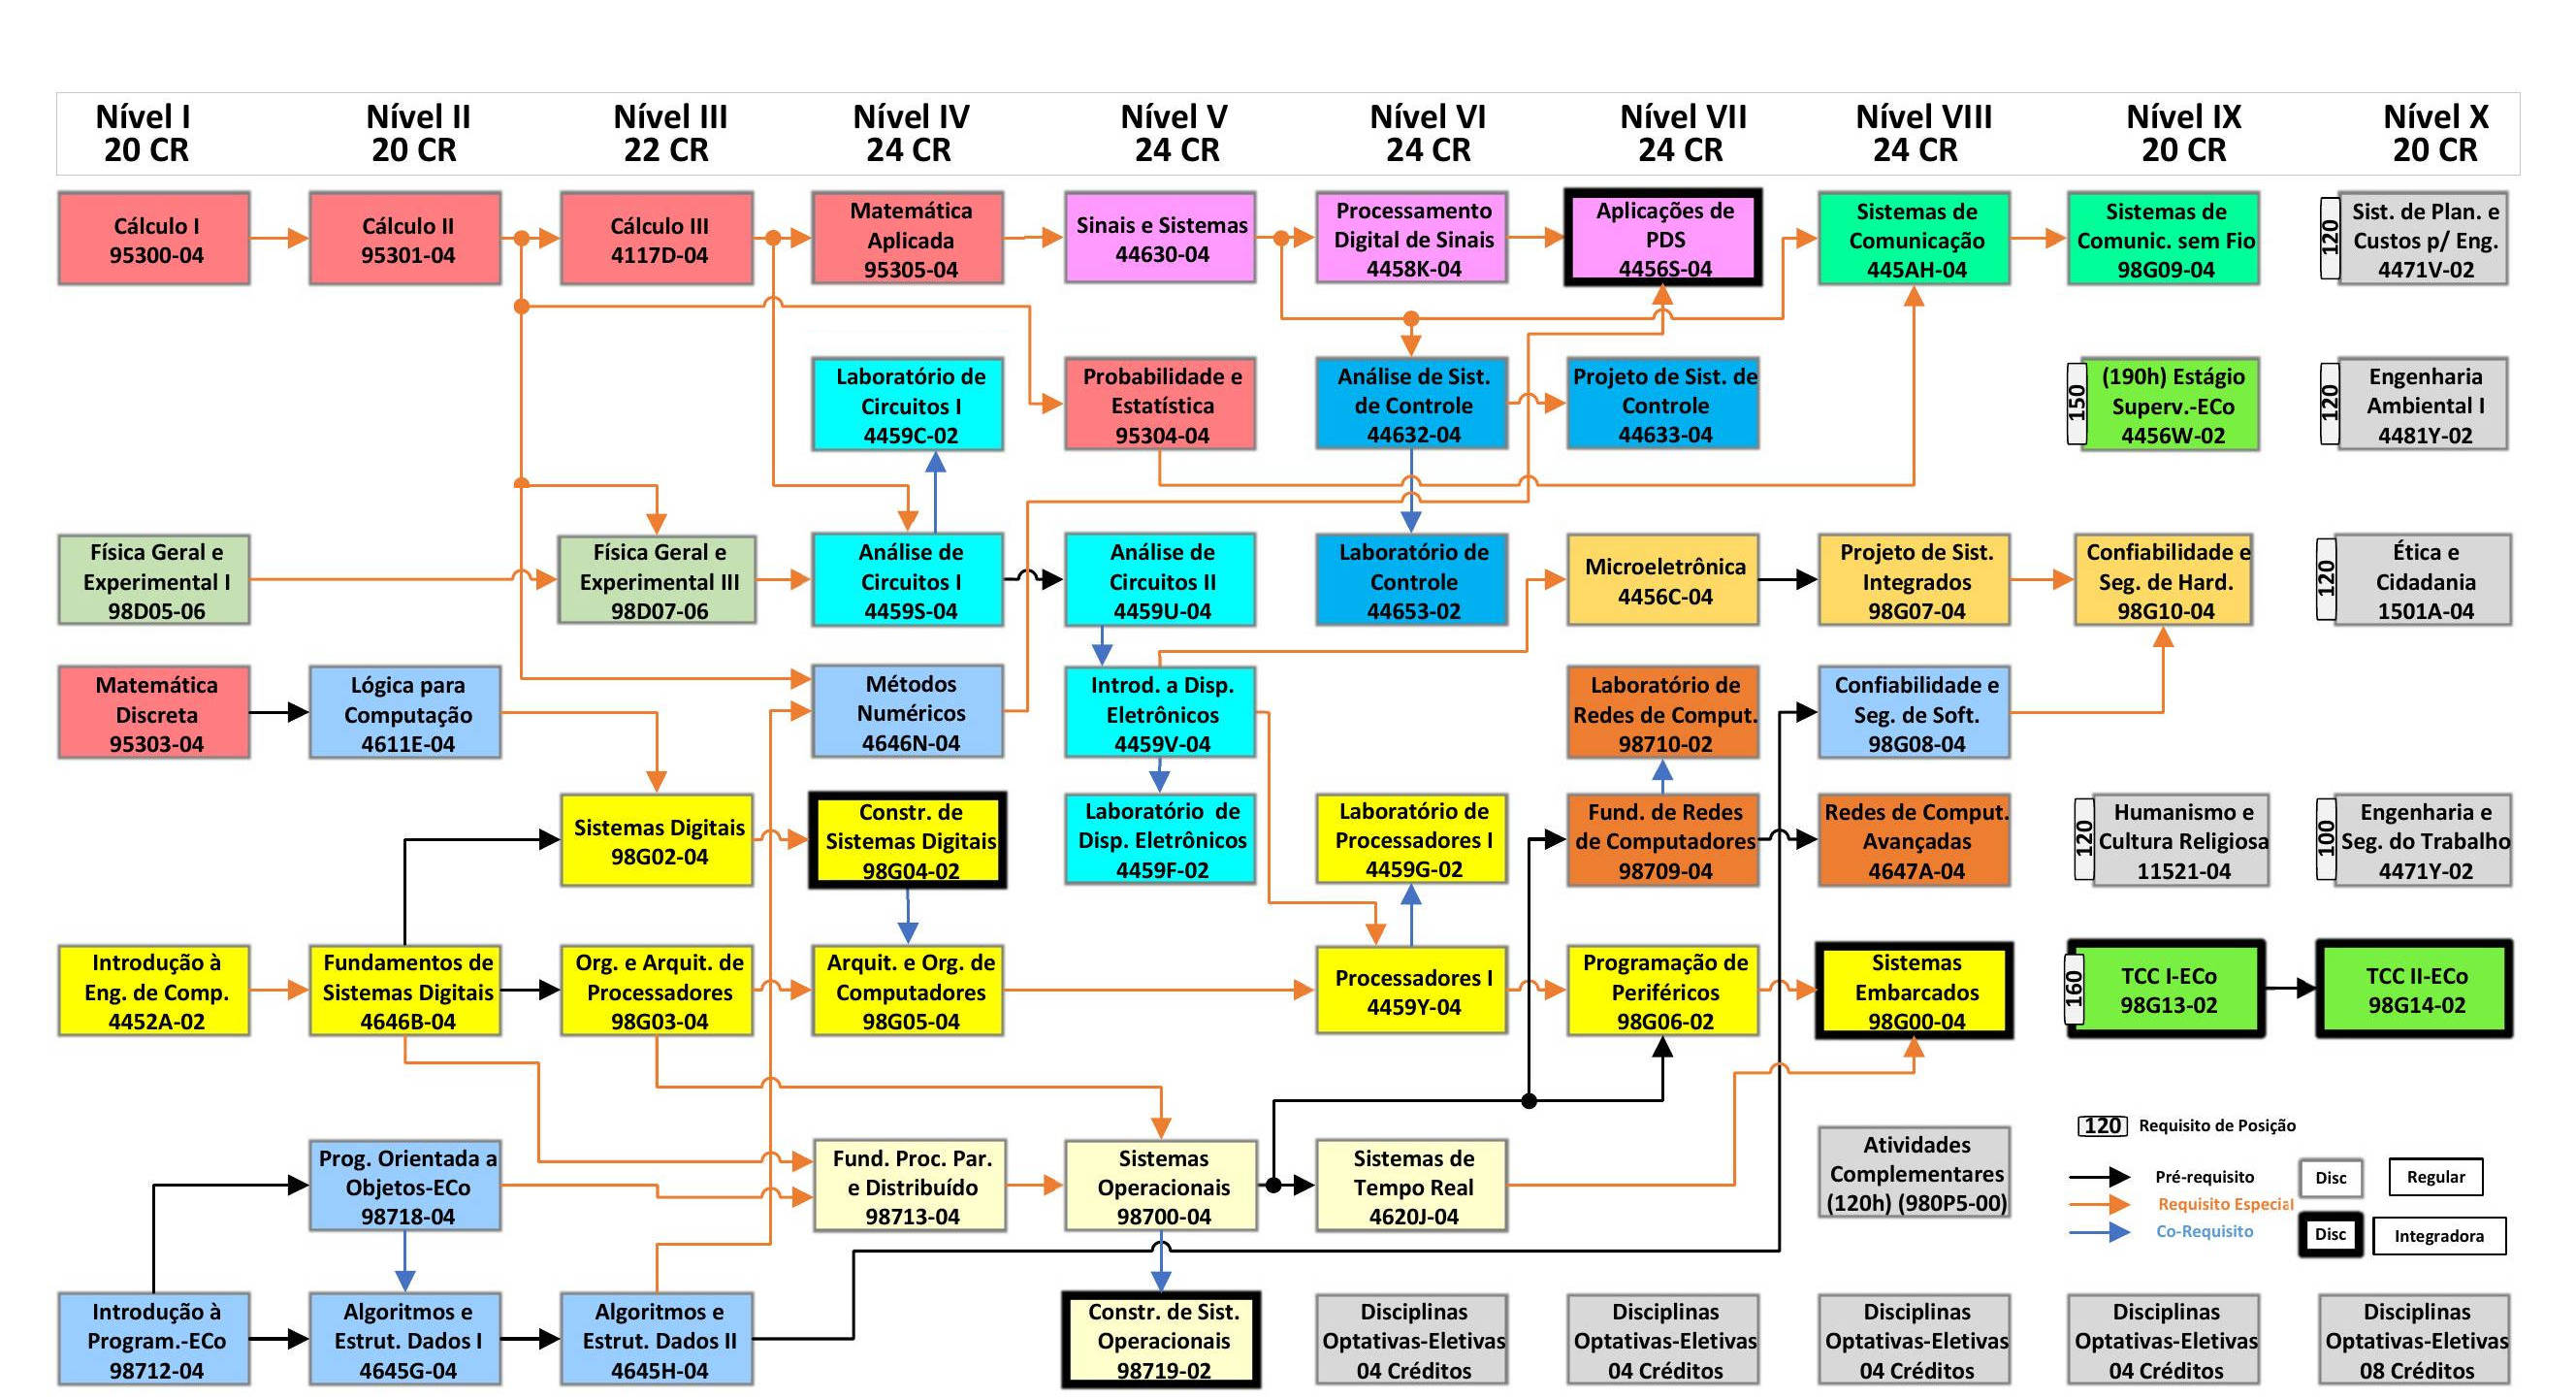
\includegraphics[width=\textwidth]{pucrs-ec-matriz-curricular.jpg} % Replace with your image path
    \end{center}
\end{frame}

\begin{frame}\frametitle{Objetivos}
O cumprimento da disciplina busca dar ao aluno, ao final do semestre, condições de:
\begin{enumerate}
	\item Conhecer e utilizar de forma precisa conceitos e termos relacionados ao paradigma de orientação a objetos.
	\item Desenvolver as competências e habilidades para a criação de sistemas de complexidade média, formado por múltiplos componentes, e expressar estas soluções na forma de um sistema de classes em uma linguagem de programação.
	\item Empregar adequadamente ponteiros para manipulação de estruturas encadeadas e memória.
	\item Construir abstrações para tipos de dados, usando os conceitos de classe, objeto-mensagem, herança e polimorfismo.
	\item Compreender os conceitos avançados em orientação a objetos.
\end{enumerate}
\end{frame}




\section{Conte\'udo}


\begin{frame}\frametitle{Ementa}
Paradigma de programação orientada a objetos; Abstração; Encapsulamento; Mensagens; Relacionamento entre classes (Composição, Referência); Parametrização de tipos (\emph{template}); Uso de Ponteiros para Estruturas Encadeadas; Fluxos de Entrada e Saída; Modularização; Herança; Polimorfismo; \emph{Standard Template Library}; Conceitos avançados em Orientação a Objetos.
\end{frame}


\begin{frame}\frametitle{Conte\'udo (1/4)}
Três grandes unidades:
\begin{itemize}
	\item Orientação a objetos básica
	\item Manipulação de dados
	\item Orientação a objetos avançada
\end{itemize}
\end{frame}


\begin{frame}\frametitle{Conte\'udo (2/4)}
\small{1. Orientação a objetos básica\\
~ 1.1. Conceitos de orientação a objetos\\
~ ~ 1.1.1. Classes e objetos\\
1.1.2. Atributos e métodos: classe e instância\\
~ 1.2. Visibilidade de atributos e métodos\\
~ 1.3. Princípios de projeto orientado a objetos\\
~ ~ 1.3.1. Mensagem\\
~ ~ 1.3.2. Abstração\\
~ ~ 1.3.3. Encapsulamento\\
~ 1.4. Detalhamento de classes\\
~ ~ 1.4.1. Relacionamento entre classes (composição, referência)\\
~ ~ 1.4.2. Construtores\\
~ ~ 1.4.3. Sobrecarga\\
~ ~ 1.4.4. Autorreferência\\
~ ~ 1.4.5. Modularização  }
\end{frame}


\begin{frame}\frametitle{Conte\'udo (3/4)}
2. Manipulação de dados\\
~ 2.1. Ponteiros\\
~ 2.2. Alocação dinâmica\\
~ 2.3. Estruturas encadeadas\\
~ 2.4. Fluxos de entrada e saída
\end{frame}


\begin{frame}\frametitle{Conte\'udo (4/4)}
3. Orientação a objetos avançada\\
~ 3.1. Generalização/especialização\\
~ ~ 3.1.1. Herança simples e múltipla\\
~ ~ 3.1.2. Hierarquia de classes\\
~ 3.2. Polimorfismo\\
~ 3.3. Tratamento de exceções\\
~ 3.4. Parametrização de tipos (\emph{template})\\
~ ~ 3.4.1. \emph{Standard Template Library} (STL)\\
~ 3.5. Conceitos avançados em Orientação a Objetos
\end{frame}


\begin{frame}\frametitle{Bibliografia Básica}
%DEITEL, HARVEY M et al. \textbf{C++}: Como Programar. Porto Alegre : Bookman, 2001.\\
%~\\
%SCHILDT, H. \textbf{C++}: the complete reference. Berkeley: McGraw Hill, 1998.
RAMNATH, S.; DATHAN, B. \textbf{Object-Oriented Analysis, Design and Implementation}: an integrated approach. 2 ed. Heidelberg: Springer, 2010. 471 p. (ou anterior)\\
~\\
WEISFELD, M. \textbf{The Object-oriented Thought Process}. 4 ed. Upper Saddle River, NJ: Addison Wesley, 2013. 336 p.\\
~\\
MEYER, B. \textbf{Object Oriented Software Construction}. 2 ed. Upper Saddle River, NJ: Prentice Hall, 1997. 1296 p.
\end{frame}


\begin{frame}\frametitle{Bibliografia Complementar}
%JAMSA, K. \textbf{Aprendendo C++}. São Paulo: Makron Books, 1999.\\
%~\\
%SCHILDT, H. \textbf{Schildt's Expert C++}. Osborne MacGrawHill, 1996.\\
%~\\
%STROUSTRUP, B. \textbf{The C++ Programming Language}. Reading: Addison-Wesley, 1997.\\
%~\\
%ZEIGLER, B. \textbf{Objects and systems}: principled design with implementations in C++ and Java. Springer, 1997.
BOOCH, G. et al. \textbf{Object-oriented Analysis and Design with Applications}. 3rd ed. Upper Saddle River, NJ: Addison Wesley, 2007. 720 p. (ou anterior)\\
%~\\
DEITEL, H. M; DEITEL, P. J. \textbf{C++}: como programar. 5 ed. São Paulo: Pearson Education do Brasil, 2006. 1208 p. (ou anterior)\\
%~\\
FARRELL, J. \textbf{An Object-oriented Approach to Programming Logic and Design}. 4 ed. Boston, MA: Cengage Learning, 2012. 560 p.\\
%~\\
GAMMA, E. et al. \textbf{Padrões de Projeto}: soluções reutilizáveis de software orientado a objetos. Porto Alegre: Bookman, 2000. 364 p.\\
%~\\
SILVA Fo., A. M. \textbf{Introdução a Programação Orientada a Objetos com C++}. Rio de Janeiro, RJ: Elsevier/Campus, 2010. 312 p.
\end{frame}


\section{Avalia\c{c}\~ao}


\begin{frame}\frametitle{Avalia\c{c}\~ao}
\[
G1 = \frac{ 2 \times MT + 4 \times P_1 + 4 \times P_2}{10}
\]
\begin{itemize}
	\item $MT$ = Média de Trabalhos
 	\item $P_1$ = Prova referente à primeira parte da disciplina
	\item $P_2$ = Prova referente a todo o conteúdo da disciplina
\end{itemize}
\end{frame}

 

\section{Informa\c{c}\~oes Gerais}


\begin{frame}\frametitle{Avisos: Presenças e Faltas}
\begin{itemize}
	\item 1 encontro = 2 presen\c{c}as ou faltas
	\item em 2024-2: 34 encontros (68 horas/aula) com presença contabilizada
	\item na semana de G2, a presença NÃO é contabilizada
	\item frequ\^encia m\'inima para aprova\c{c}\~ao: 75\%
	\item limite de faltas = 25\% de 68 = 17
	\item portanto, com 17 faltas (8 encontros e meio) o aluno está REPROVADO POR FALTAS
\end{itemize}
\end{frame}

\begin{frame}\frametitle{Avisos: Moodle}
\begin{itemize}	
	\item Avisos pelo Mural
	\item D\'uvidas pelo f\'orum
	\item Material de apoio
	\item Entrega de trabalhos e exerc\'icios
	\item Solicitações de provas pelo fórum da G1 
	\item Solicitações de provas pelo fórum da G2 
    \item Não envie mensagens por outros meios, a resposta vai demorar muito mais
\end{itemize}
\end{frame}



\begin{frame}\frametitle{Avisos: Mapas Mentais}
\begin{itemize}
	\item São uma forma de representar conhecimento sobre determinado assunto
	\item Recomenda-se fortemente que o aluno construa Mapas Mentais dos conteúdos da disciplina
	\item Os Mapas Mentais poderão ser usados nas avaliações da disciplina (com exceção das provas PS e G2)
	\item Regras:
	\begin{itemize}
		\item Um Mapa Mental por unidade do conteúdo programático
		\item NÃO incluir textos grandes e/ou copiados e colados nos nodos do mapa
		\item Cada Mapa Mental em uma folha A4 impressa
		\item Todos os Mapas Mentais devem ser entregues uma semana antes da avaliação em que serão utilizados
	\end{itemize}
	\item Mapas Conceituais também são uma alternativa interessante
\end{itemize}
\end{frame}


\begin{frame}[plain] % The 'plain' option removes default header/footer
    \begin{center}
        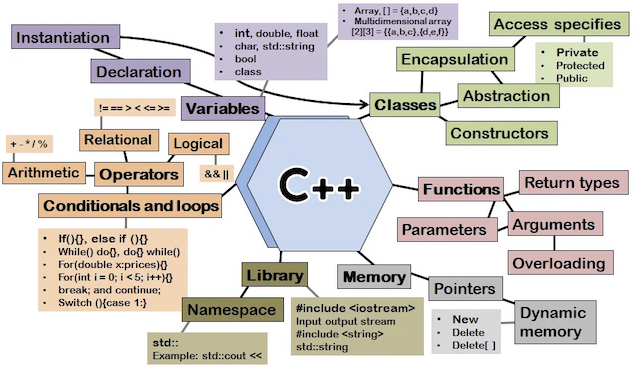
\includegraphics[width=\textwidth]{mind-map-c-plus-plus.png} % Replace with your image path
    \end{center}
\end{frame}


\begin{frame}
    \frametitle{Projetos Open Source em C++ na Exploração Espacial e Engenharia}

    \begin{itemize}
        \item \textbf{F Prime}
        \begin{itemize}
            \item Framework de software de voo usado pela NASA para sistemas de voo espacial de pequeno porte.
            \item Conceitos-chave: Sistemas embarcados, software de voo, arquitetura baseada em componentes.
            \item  \url{https://github.com/nasa/fprime}
        \end{itemize}

        \item \textbf{GMAT (General Mission Analysis Tool)}
        \begin{itemize}
            \item Ferramenta para design e navegação de missões espaciais, usada pela NASA para otimização de trajetórias.
            \item Conceitos-chave: Análise de missões espaciais, otimização de trajetórias, simulação.
            \item  \url{https://sourceforge.net/projects/gmat/}
        \end{itemize}

        \item \textbf{CFS (Core Flight System)}
        \begin{itemize}
            \item Framework de software portátil e reutilizável e conjunto de aplicativos para missões de voo espacial.
            \item Conceitos-chave: Arquitetura de software modular, aplicativos específicos de missão, componentes reutilizáveis.
            \item  \url{https://github.com/nasa/cFS}
        \end{itemize}
    \end{itemize}
\end{frame}

\begin{frame}
    \frametitle{Projetos Menores em C++ para Estudantes}

    \begin{itemize}
        \item \textbf{Tic Tac Toe}
        \begin{itemize}
            \item Jogo de console que demonstra conceitos básicos de POO.
            \item \url{https://github.com/davidschumacher/ConsoleTicTacToe} 
        \end{itemize}

        \item \textbf{CLI Sudoku Solver}
        \begin{itemize}
            \item Solucionador de Sudoku usando algoritmos de retrocesso.
            \item {\tiny\url{https://github.com/prateekiiest/Code-Sleep-Python/tree/master/Code/C++/SudokuSolver} 
            }
        \end{itemize}

        \item \textbf{Mini Motor de Busca}
        \begin{itemize}
            \item Indexa arquivos de texto e recupera resultados de busca.
            \item \url{https://github.com/AntonioNoack/Universal-Tools} 
        \end{itemize}

        \item \textbf{Servidor HTTP Simples}
        \begin{itemize}
            \item Servidor HTTP leve implementado em C++.
            \item {\tiny \url{https://github.com/cesanta/mongoose/tree/master/examples/http\_server} }
        \end{itemize}

        \item \textbf{Calculadora de Linha de Comando}
        \begin{itemize}
            \item Processa expressões matemáticas da linha de comando.
            \item \url{https://github.com/MihaiVarga/C-Expression-Evaluator}
        \end{itemize}

        \item \textbf{Traçador de Raios Básico}
        \begin{itemize}
            \item Aplicação simples de traçado de raios de luz em cenas tri-dimensionais.
            \item \url{https://github.com/ssloy/tinyraytracer} 
        \end{itemize}
    \end{itemize}
\end{frame}


\begin{frame}\frametitle{Avisos: Recomendações}
\begin{itemize}
	\item Solucione dificuldades não esclarecidas em disciplinas anteriores com aplicação e esforço extras
	\item Consulte as obras disponíveis na biblioteca (livros físicos e online)
	\item Aproveite a aula para perguntar, ler, realizar instruções e programar em C++
	\item Inicie trabalhos e exercícios imediatamente
	\item Se aprende a programar mais um pouco a cada tentativa
	\item Reserve um horário de estudo na semana para cada uma das disciplinas
	\item Procure a monitoria  
\end{itemize}
\end{frame}





\end{document}
